% topic1.tex -- Topic 1: Projectile motion, Questions 1-24.
\firsttopictitle{Topic 1 - Projectile Motion}

% ---- Q1 (acceleration at the top)
\begin{quizq}{}
A ball is kicked from the ground and follows the path shown.
\begin{center}
  \begin{tikzpicture}
    \draw[line width=0.6pt] (-0.3,0) -- (5.3,0);
    \draw[guide, domain=0:5, samples=40, smooth] plot (\x, {1.6*\x*(5-\x)/6.25});
    \fill (2.5,1.6) circle (2.5pt);
  \end{tikzpicture}
\end{center}
Which arrow represents the acceleration of the ball at its maximum height?
\opts{\tikz[baseline=-0.6ex]\draw[->, line width=0.7pt] (0,-0.25) -- (0,0.3);}
  {\tikz[baseline=-0.6ex]\draw[->, line width=0.7pt] (0,0.3) -- (0,-0.25);}
  {\tikz[baseline=-0.6ex]\draw[->, line width=0.7pt] (0,0) -- (0.55,0);}
  {Zero (there is no acceleration at this point)}
\end{quizq}

% ---- Q2 (taller bench)
\Needspace{24\baselineskip}
\begin{quizq}{}
A marble is rolled off a horizontal bench and falls to the floor.
\begin{center}
  \begin{tikzpicture}[x=0.8cm, y=0.8cm]
    \draw[line width=0.6pt] (-0.5,0) -- (6.5,0) node[below left, font=\small] {Floor};
    \draw[line width=0.6pt] (0,2.2) rectangle (2.4,2.35); \draw (0.8,0) -- (0.8,2.2); \draw (1.0,0) -- (1.0,2.2);
    \node[above, font=\small] at (0.6,2.35) {Bench};
    \shade[ball color=black!25] (2.2,2.5) circle (0.15);
    \draw[->, line width=0.6pt] (2.35,2.5) -- (2.9,2.5);
    \draw[guide, domain=2.4:5.4, samples=40, smooth] plot (\x, {2.5 - 2.5*((\x-2.4)/3.0)^2});
  \end{tikzpicture}
\end{center}
The bench is replaced by a taller bench. The marble leaves the bench with the same speed as
before.

Compared with before, what happens?
\opts{The range and the time of flight both increase.}{The range increases, but the time of flight
  stays the same.}{The time of flight increases, but the range stays the same.}{The range and the
  time of flight both stay the same.}
\end{quizq}

% ---- Q3 (speed at the highest point)
\Needspace{12\baselineskip}
\begin{quizq}{}
A video shows a kangaroo leaping from flat ground. Its take-off velocity is \qty{9.0}{m.s^{-1}} at
\ang{35} to the horizontal.

What is the speed of the kangaroo at the highest point of its leap? (Ignore air resistance.)
\opts{\qty{0}{m.s^{-1}}}{\qty{5.2}{m.s^{-1}}}{\qty{7.4}{m.s^{-1}}}{\qty{9.0}{m.s^{-1}}}
\end{quizq}

% ---- Q4 (what stays the same)
\Needspace{24\baselineskip}
\begin{quizq}{}
An object is launched from the ground and follows the path shown. $Y$ is its highest point.
\begin{center}
  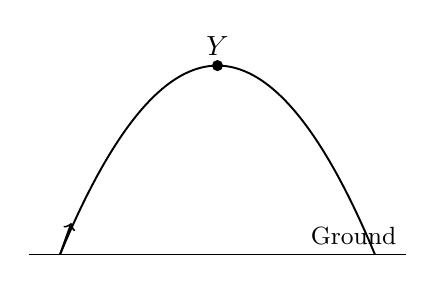
\begin{tikzpicture}[x=0.8cm, y=0.8cm]
    \draw[line width=0.6pt] (-0.5,0) -- (5.5,0) node[above left, font=\small] {Ground};
    \draw[line width=0.7pt, domain=0:5, samples=50, smooth] plot (\x, {3.0*\x*(5-\x)/6.25});
    \draw[->, line width=0.7pt] (0,0) -- (0.18,0.5);
    \fill (2.5,3.0) circle (2pt) node[above] {$Y$};
  \end{tikzpicture}
\end{center}
Which quantity is the same at launch and at point $Y$?
\opts{The horizontal component of the velocity}{The vertical component of the velocity}{The speed}
  {The kinetic energy}
\end{quizq}

% ---- Q5 (range without changing time of flight)
\Needspace{11\baselineskip}
\begin{quizq}{}
A student throws a ball that follows a parabolic path and lands at the same height.

What change to the initial velocity would make the range \emph{greater} without changing the time of
flight?
\opts{Increasing only the vertical component}{Decreasing only the vertical component}
  {Increasing only the horizontal component}{Decreasing only the horizontal component}
\end{quizq}

% ---- Q6 (dots at equal time intervals)
% Correct dots: x = 1.5 t, y = -0.5 t^2 (t = 0..4), grid units.
\Needspace{36\baselineskip}
\begin{quizq}{}
A ball is thrown horizontally from the top of a cliff. The dots show the position of the ball at
equal time intervals.

Assuming negligible air resistance, which diagram best shows the path of the ball?
\gridopts{%
  \begin{tikzpicture}[x=0.36cm, y=0.36cm]
    \draw[black!40, line width=0.3pt, xstep=0.36cm, ystep=0.36cm] (0,-9) grid (7,0);
    \fill[pattern=north east lines] (-1.2,-9) rectangle (0,0); \draw (-1.2,0) -- (0,0) -- (0,-9);
    \foreach \x/\y in {0/0, 1.5/-2, 3/-4, 4.5/-6, 6/-8} \fill[black!60] (\x,\y) circle (3.5pt);
  \end{tikzpicture}}
  {%
  \begin{tikzpicture}[x=0.36cm, y=0.36cm]
    \draw[black!40, line width=0.3pt, xstep=0.36cm, ystep=0.36cm] (0,-9) grid (7,0);
    \fill[pattern=north east lines] (-1.2,-9) rectangle (0,0); \draw (-1.2,0) -- (0,0) -- (0,-9);
    \foreach \x/\y in {0/0, 1.5/-0.5, 3/-2, 4.5/-4.5, 6/-8} \fill[black!60] (\x,\y) circle (3.5pt);
  \end{tikzpicture}}
  {%
  \begin{tikzpicture}[x=0.36cm, y=0.36cm]
    \draw[black!40, line width=0.3pt, xstep=0.36cm, ystep=0.36cm] (0,-9) grid (7,0);
    \fill[pattern=north east lines] (-1.2,-9) rectangle (0,0); \draw (-1.2,0) -- (0,0) -- (0,-9);
    \foreach \x/\y in {0/0, 2.5/-0.5, 4.5/-2, 5.5/-4.5, 6/-8} \fill[black!60] (\x,\y) circle (3.5pt);
  \end{tikzpicture}}
  {%
  \begin{tikzpicture}[x=0.36cm, y=0.36cm]
    \draw[black!40, line width=0.3pt, xstep=0.36cm, ystep=0.36cm] (0,-9) grid (7,0);
    \fill[pattern=north east lines] (-1.2,-9) rectangle (0,0); \draw (-1.2,0) -- (0,0) -- (0,-9);
    \foreach \x/\y in {0/0, 1.5/-3.5, 3/-6, 4.5/-7.5, 6/-8} \fill[black!60] (\x,\y) circle (3.5pt);
  \end{tikzpicture}}
\end{quizq}

% ---- Q7 (components of the acceleration)
\Needspace{22\baselineskip}
\begin{quizq}{}
A cannonball is fired from a cannon and follows a parabolic path. Consider four points along its
path, from just after launch to just before landing. Ignore air resistance.

Which set of vectors represents the horizontal and vertical components of the cannonball's
\emph{acceleration} at these four points?
\begin{center}
  \renewcommand\arraystretch{1.8}
  \begin{tabular}{@{}p{10mm}|*{4}{>{\centering\arraybackslash}p{9mm}}|*{4}{>{\centering\arraybackslash}p{9mm}}|}
    \cline{2-9}
    & \multicolumn{4}{c|}{\textit{Horizontal}} & \multicolumn{4}{c|}{\textit{Vertical}}\\ \cline{2-9}
    A. & \ra & \ra & \ra & \ra & \da & \da & \da & \da\\ \cline{2-9}
    B. & 0 & 0 & 0 & 0 & \ua & \ua & \da & \da\\ \cline{2-9}
    C. & 0 & 0 & 0 & 0 & \da & \da & \da & \da\\ \cline{2-9}
    D. & \ra & \ra & \ra & \ra & \ua & \ua & \da & \da\\ \cline{2-9}
  \end{tabular}
\end{center}
\end{quizq}

% ---- Q8 (hits a wall on the way down)
\Needspace{26\baselineskip}
\begin{quizq}{}
An object is launched from the ground with an initial velocity $u$. It hits a wall with velocity
$v$ while it is moving downwards.
\begin{center}
  \begin{tikzpicture}[x=0.8cm, y=0.8cm]
    \draw[line width=0.6pt] (-0.5,0) -- (6.4,0);
    \fill[black!20] (5,0) rectangle (5.9,3.6); \draw (5,0) rectangle (5.9,3.6);
    \node[font=\small] at (5.45,2.8) {Wall};
    \draw[guide, domain=0:5, samples=50, smooth] plot (\x, {3.0*\x*(6.6-\x)/10.89});
    \draw[->, line width=0.7pt] (0,0) -- (0.3,0.55) node[left, font=\small] {$u$};
    \draw[->, line width=0.7pt] (4.62,2.52) -- (4.92,2.30) node[above=3pt, font=\small] {$v$};
  \end{tikzpicture}
\end{center}
Which statement correctly compares the components of $u$ and $v$? Ignore air resistance.
\opts{The horizontal component of $v$ is equal to the horizontal component of $u$.}
  {The horizontal component of $v$ is less than the horizontal component of $u$.}
  {The vertical component of $v$ is upwards.}
  {The vertical component of $v$ is greater in size than the vertical component of $u$.}
\end{quizq}

% ---- Q9 (dropped and launched horizontally)
\Needspace{14\baselineskip}
\begin{quizq}{}
Two identical balls, X and Y, are at the same height above level ground. At the same instant, ball
X is dropped from rest and ball Y is launched horizontally.

Which statement correctly describes what happens? (Ignore air resistance.)
\opts{X hits the ground first, because it travels a shorter distance.}
  {Y hits the ground first, because it has a greater speed.}
  {X and Y hit the ground at the same time, with the same speed.}
  {X and Y hit the ground at the same time, but Y has a greater speed.}
\end{quizq}

% ---- Q10 (x-t and y-t graphs)
\Needspace{40\baselineskip}
\begin{quizq}{}
A ball is launched at an angle above level ground. $x$ is its horizontal displacement and $y$ is its
vertical displacement (upwards is positive).

Which pair of graphs best represents the motion of the ball until it lands?
\pairopts{%
  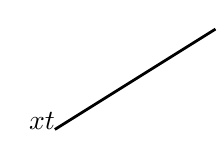
\begin{tikzpicture}[scale=0.85]\gaxesP{$x$}{$t$}
    \draw[line width=1pt] (0,0) -- (2.4,1.5);
  \end{tikzpicture}}{%
  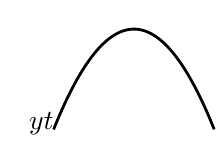
\begin{tikzpicture}[scale=0.85]\gaxesP{$y$}{$t$}
    \draw[line width=1pt, domain=0:2.4, samples=40, smooth] plot (\x, {1.5*\x*(2.4-\x)/1.44});
  \end{tikzpicture}}
  {%
  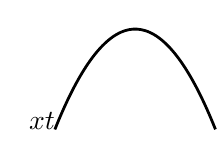
\begin{tikzpicture}[scale=0.85]\gaxesP{$x$}{$t$}
    \draw[line width=1pt, domain=0:2.4, samples=40, smooth] plot (\x, {1.5*\x*(2.4-\x)/1.44});
  \end{tikzpicture}}{%
  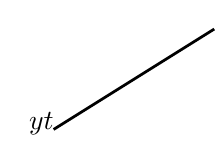
\begin{tikzpicture}[scale=0.85]\gaxesP{$y$}{$t$}
    \draw[line width=1pt] (0,0) -- (2.4,1.5);
  \end{tikzpicture}}
  {%
  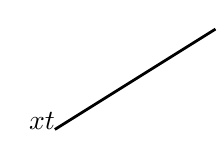
\begin{tikzpicture}[scale=0.85]\gaxesP{$x$}{$t$}
    \draw[line width=1pt] (0,0) -- (2.4,1.5);
  \end{tikzpicture}}{%
  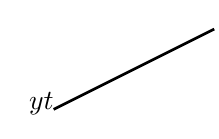
\begin{tikzpicture}[scale=0.85]\gaxesP{$y$}{$t$}
    \draw[line width=1pt] (0,0) -- (2.4,1.2);
  \end{tikzpicture}}
  {%
  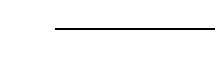
\begin{tikzpicture}[scale=0.85]\gaxesP{$x$}{$t$}
    \draw[line width=1pt] (0,1.0) -- (2.4,1.0);
  \end{tikzpicture}}{%
  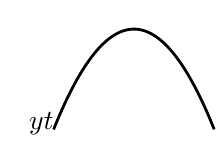
\begin{tikzpicture}[scale=0.85]\gaxesP{$y$}{$t$}
    \draw[line width=1pt, domain=0:2.4, samples=40, smooth] plot (\x, {1.5*\x*(2.4-\x)/1.44});
  \end{tikzpicture}}
\end{quizq}

% ---- Q11 (down is positive: v-t and a-t)
\Needspace{44\baselineskip}
\begin{quizq}{}
A ball is thrown vertically upwards and is caught when it returns to the same height.

Taking \emph{downwards} as the positive direction, which pair of graphs best describes the
velocity, $v$, and acceleration, $a$, of the ball as functions of time, $t$? Ignore air resistance.
\pairopts{%
  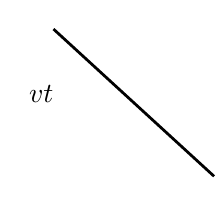
\begin{tikzpicture}[scale=0.85]\gaxesPN{$v$}{$t$}
    \draw[line width=1pt] (0,1.1) -- (2.4,-1.1);
  \end{tikzpicture}}{%
  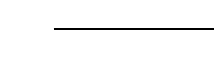
\begin{tikzpicture}[scale=0.85]\gaxesPN{$a$}{$t$}
    \draw[line width=1pt] (0,-0.8) -- (2.4,-0.8);
  \end{tikzpicture}}
  {%
  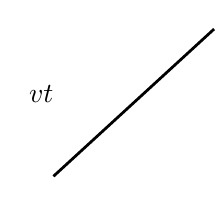
\begin{tikzpicture}[scale=0.85]\gaxesPN{$v$}{$t$}
    \draw[line width=1pt] (0,-1.1) -- (2.4,1.1);
  \end{tikzpicture}}{%
  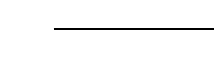
\begin{tikzpicture}[scale=0.85]\gaxesPN{$a$}{$t$}
    \draw[line width=1pt] (0,0.8) -- (2.4,0.8);
  \end{tikzpicture}}
  {%
  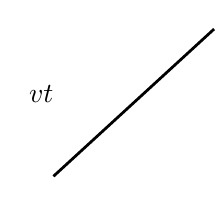
\begin{tikzpicture}[scale=0.85]\gaxesPN{$v$}{$t$}
    \draw[line width=1pt] (0,-1.1) -- (2.4,1.1);
  \end{tikzpicture}}{%
  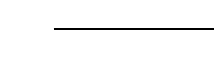
\begin{tikzpicture}[scale=0.85]\gaxesPN{$a$}{$t$}
    \draw[line width=1pt] (0,-0.8) -- (2.4,-0.8);
  \end{tikzpicture}}
  {%
  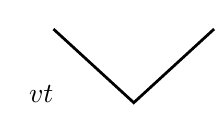
\begin{tikzpicture}[scale=0.85]\gaxesPN{$v$}{$t$}
    \draw[line width=1pt] (0,1.1) -- (1.2,0) -- (2.4,1.1);
  \end{tikzpicture}}{%
  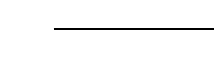
\begin{tikzpicture}[scale=0.85]\gaxesPN{$a$}{$t$}
    \draw[line width=1pt] (0,0.8) -- (2.4,0.8);
  \end{tikzpicture}}
\end{quizq}

% ---- Q12 (gravitational potential energy during flight)
\Needspace{30\baselineskip}
\begin{quizq}{}
A ball is thrown upwards at an angle of \ang{45}. It lands at the same height as it was thrown from.

Which graph best represents the gravitational potential energy $E_\mathrm{p}$ of the ball during its
time of flight? ($E_\mathrm{p} = 0$ at the launch height.)
\gridopts{%
  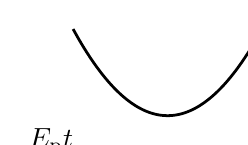
\begin{tikzpicture}\gaxesP{$E_\mathrm{p}$}{$t$}
    \draw[line width=1pt, domain=0:2.4, samples=40, smooth] plot (\x, {1.5 - 1.1*\x*(2.4-\x)/1.44});
  \end{tikzpicture}}
  {%
  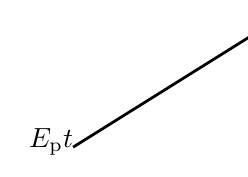
\begin{tikzpicture}\gaxesP{$E_\mathrm{p}$}{$t$}
    \draw[line width=1pt] (0,0) -- (2.4,1.5);
  \end{tikzpicture}}
  {%
  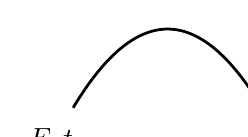
\begin{tikzpicture}\gaxesP{$E_\mathrm{p}$}{$t$}
    \draw[line width=1pt, domain=0:2.4, samples=40, smooth] plot (\x, {0.5 + 1.0*\x*(2.4-\x)/1.44});
  \end{tikzpicture}}
  {%
  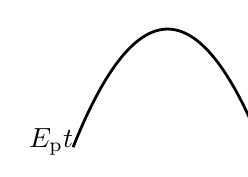
\begin{tikzpicture}\gaxesP{$E_\mathrm{p}$}{$t$}
    \draw[line width=1pt, domain=0:2.4, samples=40, smooth] plot (\x, {1.5*\x*(2.4-\x)/1.44});
  \end{tikzpicture}}
\end{quizq}

% ---- Q13 (from v-t graph to displacement-time graph)
\Needspace{40\baselineskip}
\begin{quizq}{}
A projectile is launched vertically upwards. Its velocity as a function of time is shown (upwards
is positive).
\begin{center}
  \begin{tikzpicture}
    \draw[axisline] (0,0) -- (3.4,0) node[right, font=\small] {Time (s)};
    \draw[axisline] (0,-1.4) -- (0,1.6) node[above, font=\small] {Velocity (\si{m.s^{-1}})};
    \draw[line width=1pt] (0,1.2) -- (2.8,-1.2);
    \foreach \x/\l in {0.7/1, 1.4/2, 2.1/3, 2.8/4} {\draw (\x,0.06) -- (\x,-0.06); \node[below, font=\footnotesize] at (\x,-0.06) {\l};}
    \node[left, font=\footnotesize] at (0,1.2) {19.6}; \node[left, font=\footnotesize] at (0,-1.2) {$-19.6$};
    \draw[guide] (0,-1.2) -- (2.8,-1.2);
  \end{tikzpicture}
\end{center}
Which displacement--time graph corresponds to this motion?
\gridopts{%
  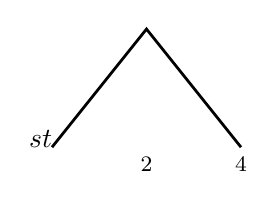
\begin{tikzpicture}\gaxesP{$s$}{$t$}
    \draw[line width=1pt] (0,0) -- (1.2,1.5) -- (2.4,0);
    \node[below, font=\footnotesize] at (1.2,0) {2}; \node[below, font=\footnotesize] at (2.4,0) {4};
  \end{tikzpicture}}
  {%
  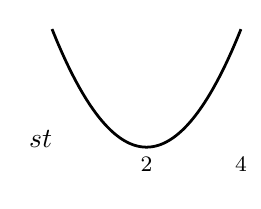
\begin{tikzpicture}\gaxesP{$s$}{$t$}
    \draw[line width=1pt, domain=0:2.4, samples=40, smooth] plot (\x, {1.5 - 1.5*\x*(2.4-\x)/1.44});
    \node[below, font=\footnotesize] at (1.2,0) {2}; \node[below, font=\footnotesize] at (2.4,0) {4};
  \end{tikzpicture}}
  {%
  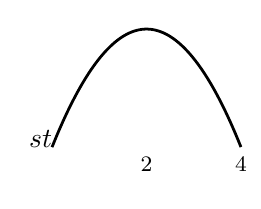
\begin{tikzpicture}\gaxesP{$s$}{$t$}
    \draw[line width=1pt, domain=0:2.4, samples=40, smooth] plot (\x, {1.5*\x*(2.4-\x)/1.44});
    \node[below, font=\footnotesize] at (1.2,0) {2}; \node[below, font=\footnotesize] at (2.4,0) {4};
  \end{tikzpicture}}
  {%
  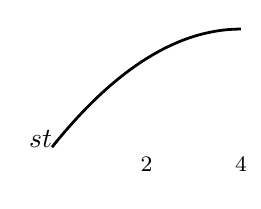
\begin{tikzpicture}\gaxesP{$s$}{$t$}
    \draw[line width=1pt, domain=0:2.4, samples=40, smooth] plot (\x, {1.5*\x*(4.8-\x)/5.76});
    \node[below, font=\footnotesize] at (1.2,0) {2}; \node[below, font=\footnotesize] at (2.4,0) {4};
  \end{tikzpicture}}
\end{quizq}

% ---- Q14 (launch angle from maximum height)
\Needspace{12\baselineskip}
\begin{quizq}{}
A cannonball is launched at \qty{40}{m.s^{-1}}. It reaches a maximum height of \qty{60}{m} above
its launch point.

To the nearest degree, what is the angle of elevation of the launch?
\opts{\ang{31}}{\ang{45}}{\ang{56}}{\ang{59}}
\end{quizq}

% ---- Q15 (range against launch angle)
\Needspace{30\baselineskip}
\begin{quizq}{}
A ball is launched from level ground with the same speed each time, at different launch angles
between \ang{0} and \ang{90}.

Which graph correctly represents the relationship between launch angle and range?
\gridopts{%
  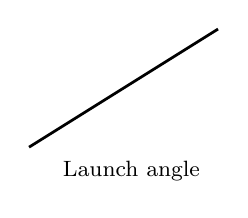
\begin{tikzpicture}\gaxesP{Range}{}
    \draw[line width=1pt] (0,0) -- (2.4,1.5);
    \node[below, font=\footnotesize] at (1.3,-0.05) {Launch angle};
  \end{tikzpicture}}
  {%
  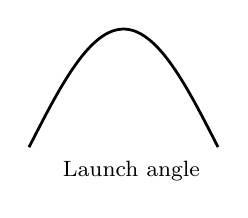
\begin{tikzpicture}\gaxesP{Range}{}
    \draw[line width=1pt, domain=0:2.4, samples=60, smooth] plot (\x, {1.5*sin(75*\x)});
    \node[below, font=\footnotesize] at (1.3,-0.05) {Launch angle};
  \end{tikzpicture}}
  {%
  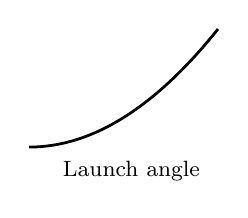
\begin{tikzpicture}\gaxesP{Range}{}
    \draw[line width=1pt, domain=0:2.4, samples=60, smooth] plot (\x, {1.5*(\x/2.4)^2});
    \node[below, font=\footnotesize] at (1.3,-0.05) {Launch angle};
  \end{tikzpicture}}
  {%
  
\begin{tikzpicture}\gaxesP{Range}{}
    \draw[line width=1pt] (0,0.9) -- (2.4,0.9);
    \node[below, font=\footnotesize] at (1.3,-0.05) {Launch angle};
  \end{tikzpicture}}
\end{quizq}

% ---- Q16 (speed when the velocity is at 30 degrees)
\Needspace{12\baselineskip}
\begin{quizq}{}
A ball is launched horizontally from a cliff. After 1.5 seconds, the ball's velocity is directed at
\ang{30} below the horizontal.

What is the magnitude of the velocity, in \si{m.s^{-1}}, at 1.5 seconds?
\opts{14.7}{17.0}{25.5}{29.4}
\end{quizq}

% ---- Q17 (energy statements)
\Needspace{26\baselineskip}
\begin{quizq}{}
An object is launched from the ground and follows the path shown. $Y$ is its highest point. Ignore
air resistance.
\begin{center}
  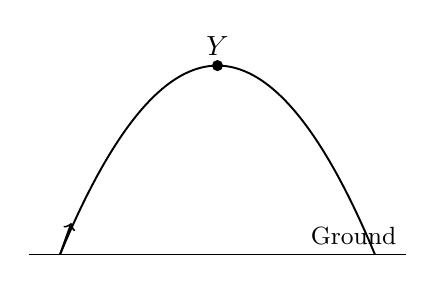
\begin{tikzpicture}[x=0.8cm, y=0.8cm]
    \draw[line width=0.6pt] (-0.5,0) -- (5.5,0) node[above left, font=\small] {Ground};
    \draw[line width=0.7pt, domain=0:5, samples=50, smooth] plot (\x, {3.0*\x*(5-\x)/6.25});
    \draw[->, line width=0.7pt] (0,0) -- (0.18,0.5);
    \fill (2.5,3.0) circle (2pt) node[above] {$Y$};
  \end{tikzpicture}
\end{center}
Choose the most correct statement.
\opts{The kinetic energy at point $Y$ is zero.}
  {The gravitational potential energy at point $Y$ is a minimum.}
  {The total mechanical energy at point $Y$ is greater than at launch.}
  {The kinetic energy at point $Y$ is the smallest kinetic energy of the flight, but it is not zero.}
\end{quizq}

% ---- Q18 (bus speeding up: frame of reference)
\Needspace{26\baselineskip}
\begin{quizq}{}
A mass hangs on a string from the roof of a bus. The bus is travelling forward on a horizontal road
at a constant velocity.
\begin{center}
  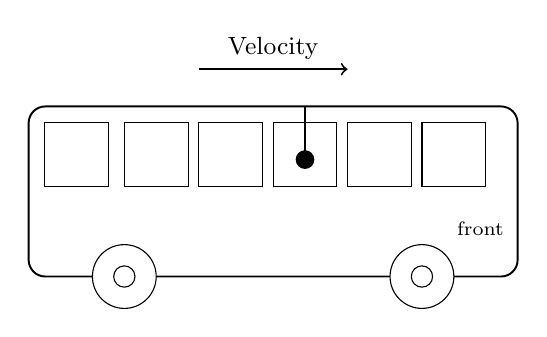
\begin{tikzpicture}[scale=1.35]
    \draw[rounded corners=6pt, line width=0.7pt] (0,0.3) rectangle (4.6,1.9);
    \foreach \x in {0.9,1.6,2.3,3.0,3.7} \draw (\x,1.15) rectangle (\x+0.6,1.75);
    \draw (0.15,1.15) rectangle (0.75,1.75);
    \draw (2.6,1.9) -- (2.6,1.45); \fill (2.6,1.4) circle (2.5pt);
    \foreach \x in {0.9,3.7} {\draw[fill=white] (\x,0.3) circle (0.3); \draw (\x,0.3) circle (0.1);}
    \draw[->, line width=0.7pt] (1.6,2.25) -- (3.0,2.25) node[midway, above, font=\small] {Velocity};
    \node[font=\scriptsize] at (4.25,0.75) {front};
  \end{tikzpicture}
\end{center}
The string holding the mass is cut. At the same instant, the driver presses the accelerator, and
the bus speeds up at a rate of \qty{2}{m.s^{-2}}.

Which statement correctly describes the motion of the mass, as observed from within the frame of
reference of the bus?
\opts{The mass travels in a straight line vertically downwards.}
  {The mass travels in a straight line downwards and towards the front of the bus.}
  {The mass travels in a straight line downwards and towards the back of the bus.}
  {The mass travels in a parabolic path downwards and towards the back of the bus.}
\end{quizq}

% ---- Q19 (rocket: thrust less than weight)
% Weight 49 000 N > thrust 40 000 N: net force 9000 N down, so the path curves downwards.
\Needspace{40\baselineskip}
\begin{quizq}{}
A rocket of mass \qty{5000}{kg} is travelling horizontally at \qty{15}{m.s^{-1}} above the ground.
Its engine pushes vertically upwards. The engine thrust is then changed to \qty{40000}{N}.

Which diagram shows the path of the rocket after this change of thrust?
\gridopts{%
  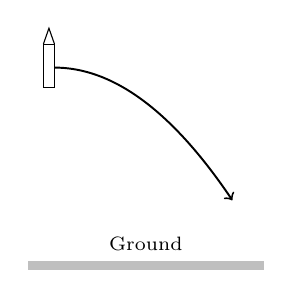
\begin{tikzpicture}
    \fill[black!25] (0,-0.12) rectangle (3,0); \node[above, font=\scriptsize] at (1.5,0) {Ground};
    \draw[fill=white] (0.2,2.2) rectangle (0.34,2.75); \draw[fill=white] (0.2,2.75) -- (0.27,2.95) -- (0.34,2.75);
    \draw[->, line width=0.7pt, domain=0.34:2.6, samples=40, smooth] plot (\x, {2.45 - 0.33*(\x-0.34)^2});
  \end{tikzpicture}}
  {%
  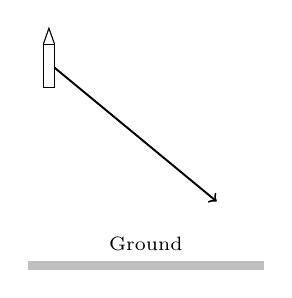
\begin{tikzpicture}
    \fill[black!25] (0,-0.12) rectangle (3,0); \node[above, font=\scriptsize] at (1.5,0) {Ground};
    \draw[fill=white] (0.2,2.2) rectangle (0.34,2.75); \draw[fill=white] (0.2,2.75) -- (0.27,2.95) -- (0.34,2.75);
    \draw[->, line width=0.7pt] (0.34,2.45) -- (2.4,0.75);
  \end{tikzpicture}}
  {%
  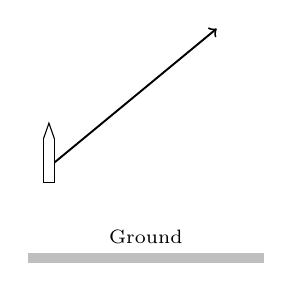
\begin{tikzpicture}
    \fill[black!25] (0,-0.12) rectangle (3,0); \node[above, font=\scriptsize] at (1.5,0) {Ground};
    \draw[fill=white] (0.2,0.9) rectangle (0.34,1.45); \draw[fill=white] (0.2,1.45) -- (0.27,1.65) -- (0.34,1.45);
    \draw[->, line width=0.7pt] (0.34,1.15) -- (2.4,2.85);
  \end{tikzpicture}}
  {%
  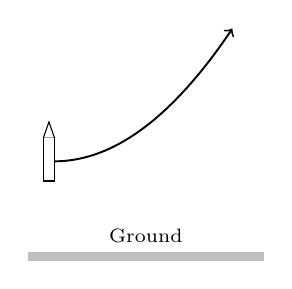
\begin{tikzpicture}
    \fill[black!25] (0,-0.12) rectangle (3,0); \node[above, font=\scriptsize] at (1.5,0) {Ground};
    \draw[fill=white] (0.2,0.9) rectangle (0.34,1.45); \draw[fill=white] (0.2,1.45) -- (0.27,1.65) -- (0.34,1.45);
    \draw[->, line width=0.7pt, domain=0.34:2.6, samples=40, smooth] plot (\x, {1.15 + 0.33*(\x-0.34)^2});
  \end{tikzpicture}}
\end{quizq}

% ---- Q20 (lift slowing down while moving downwards)
% Lift accelerates upwards, so the effective g is bigger: the path curves down more steeply.
\Needspace{44\baselineskip}
\begin{quizq}{}
A projectile was launched horizontally inside a lift. The diagram shows the path of the
projectile when the lift was stationary.
\begin{center}
  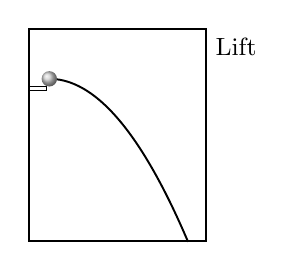
\begin{tikzpicture}[scale=0.75]
    \draw[line width=0.7pt] (0,0) rectangle (3,3.6); \node[right, font=\small] at (3,3.3) {Lift};
    \draw (0,2.55) rectangle (0.3,2.62);
    \draw[line width=0.7pt, domain=0.35:2.7, samples=40, smooth] plot (\x, {2.75 - 0.5*(\x-0.35)^2});
    \shade[ball color=black!20] (0.35,2.75) circle (0.13);
  \end{tikzpicture}
\end{center}
The projectile was launched again with the same velocity. This time, the lift was moving
\emph{downwards} and slowing down as it approached the ground floor.

Which diagram correctly shows the new path of the projectile (dotted line) relative to the path in
the stationary lift (solid line)?
\gridopts{%
  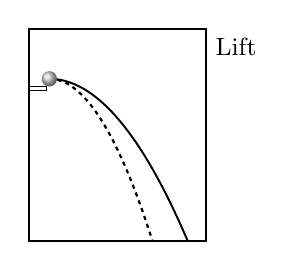
\begin{tikzpicture}[scale=0.75]
    \draw[line width=0.7pt] (0,0) rectangle (3,3.6); \node[right, font=\small] at (3,3.3) {Lift};
    \draw (0,2.55) rectangle (0.3,2.62);
    \draw[line width=0.7pt, domain=0.35:2.7, samples=40, smooth] plot (\x, {2.75 - 0.5*(\x-0.35)^2});
    \draw[line width=0.8pt, dash pattern=on 1.5pt off 1.5pt, domain=0.35:2.1, samples=40, smooth] plot (\x, {2.75 - 0.9*(\x-0.35)^2});
    \shade[ball color=black!20] (0.35,2.75) circle (0.13);
  \end{tikzpicture}}
  {%
  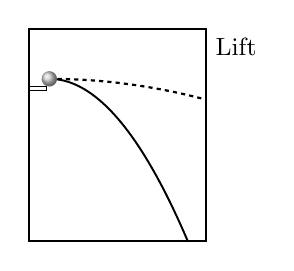
\begin{tikzpicture}[scale=0.75]
    \draw[line width=0.7pt] (0,0) rectangle (3,3.6); \node[right, font=\small] at (3,3.3) {Lift};
    \draw (0,2.55) rectangle (0.3,2.62);
    \draw[line width=0.7pt, domain=0.35:2.7, samples=40, smooth] plot (\x, {2.75 - 0.5*(\x-0.35)^2});
    \draw[line width=0.8pt, dash pattern=on 1.5pt off 1.5pt, domain=0.35:3, samples=40, smooth] plot (\x, {2.75 - 0.05*(\x-0.35)^2});
    \shade[ball color=black!20] (0.35,2.75) circle (0.13);
  \end{tikzpicture}}
  {%
  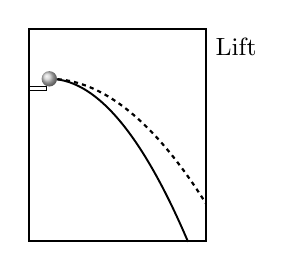
\begin{tikzpicture}[scale=0.75]
    \draw[line width=0.7pt] (0,0) rectangle (3,3.6); \node[right, font=\small] at (3,3.3) {Lift};
    \draw (0,2.55) rectangle (0.3,2.62);
    \draw[line width=0.7pt, domain=0.35:2.7, samples=40, smooth] plot (\x, {2.75 - 0.5*(\x-0.35)^2});
    \draw[line width=0.8pt, dash pattern=on 1.5pt off 1.5pt, domain=0.35:3, samples=40, smooth] plot (\x, {2.75 - 0.3*(\x-0.35)^2});
    \shade[ball color=black!20] (0.35,2.75) circle (0.13);
  \end{tikzpicture}}
  {%
  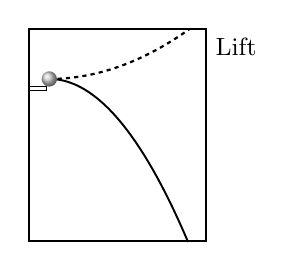
\begin{tikzpicture}[scale=0.75]
    \draw[line width=0.7pt] (0,0) rectangle (3,3.6); \node[right, font=\small] at (3,3.3) {Lift};
    \draw (0,2.55) rectangle (0.3,2.62);
    \draw[line width=0.7pt, domain=0.35:2.7, samples=40, smooth] plot (\x, {2.75 - 0.5*(\x-0.35)^2});
    \draw[line width=0.8pt, dash pattern=on 1.5pt off 1.5pt, domain=0.35:2.73, samples=40, smooth] plot (\x, {2.75 + 0.15*(\x-0.35)^2});
    \shade[ball color=black!20] (0.35,2.75) circle (0.13);
  \end{tikzpicture}}
\end{quizq}

% ---- Q21 (range on level ground)
\Needspace{12\baselineskip}
\begin{quizq}{}
A ball is kicked from level ground at \qty{25}{m.s^{-1}} at \ang{40} above the horizontal. It lands
at the same height. What is its range?
\opts{\qty{31.4}{m}}{\qty{52.7}{m}}{\qty{62.8}{m}}{\qty{63.8}{m}}
\end{quizq}

% ---- Q22 (maximum height)
\Needspace{12\baselineskip}
\begin{quizq}{}
A ball is launched at \qty{30}{m.s^{-1}} at \ang{50} above the horizontal. What is the maximum height
it reaches above its launch point?
\opts{\qty{19.0}{m}}{\qty{26.9}{m}}{\qty{45.9}{m}}{\qty{53.9}{m}}
\end{quizq}

% ---- Q23 (horizontal launch from a cliff)
\Needspace{12\baselineskip}
\begin{quizq}{}
A stone is thrown horizontally at \qty{12}{m.s^{-1}} from the top of a cliff \qty{45}{m} high. How far
from the base of the cliff does it land?
\opts{\qty{25.7}{m}}{\qty{36.4}{m}}{\qty{45.0}{m}}{\qty{356}{m}}
\end{quizq}

% ---- Q24 (launched upwards from a cliff: time of flight)
\Needspace{13\baselineskip}
\begin{quizq}{}
A ball is launched at \qty{15}{m.s^{-1}} at \ang{30} \emph{above} the horizontal from the top of a cliff
\qty{40}{m} high. It lands on the flat ground at the base of the cliff.

What is its time of flight?
\opts{\qty{1.53}{s}}{\qty{2.19}{s}}{\qty{2.86}{s}}{\qty{3.72}{s}}
\end{quizq}
